\documentclass[conference]{IEEEtran}
\usepackage{stmaryrd}
\usepackage{amsfonts}
% If the IEEEtran.cls has not been installed into the LaTeX system files,
% manually specify the path to it: e.g.,
% \documentclass[conference]{../sty/IEEEtran}

\usepackage{graphicx,times,amsmath,multi row} % Add all your packages here

% correct bad hyphenation here
\hyphenation{op-tical net-works semi-conduc-tor IEEEtran}

\IEEEoverridecommandlockouts    % to create the author's affliation portion
                % using \thanks

\textwidth 178mm    % <------ These are the adjustments we made 10/18/2005
\textheight 239mm   % You may or may not need to adjust these numbes again
\oddsidemargin -7mm
\evensidemargin -7mm
\topmargin -6mm
\columnsep 5mm

% -------- The above  is from IEEE Sample.tex
%\usepackage{geometry}                % See geometry.pdf to learn the layout options. There are lots.
%\geometry{letterpaper}                   % ... or a4paper or a5paper or ... 
%\geometry{landscape}                % Activate for for rotated page geometry
%\usepackage[parfill]{parskip}    % Activate to begin paragraphs with an empty line rather than an indent
\usepackage{graphicx}
\usepackage{amssymb}
%\usepackage{epstopdf}
%\DeclareGraphicsRule{.tif}{png}{.png}{`convert #1 `dirname #1`/`basename #1 .tif`.png}
%\usepackage{amsmath,amsthm}
\usepackage{times}
\usepackage{color}
%\usepackage[pagewise]{lineno}

%\newcommand{\spacedouble}{\renewcommand{\baselinestretch}{0.95}\Huge\normalsize}
%\newcommand{\spacesingle}{\renewcommand{\baselinestretch}{1.0}\Huge\normalsize}
\newcommand{\cA}{{\cal A}}
\newcommand{\cD}{{\cal D}}
\newcommand{\cL}{{\cal L}}
\newcommand{\cP}{{\cal P}}
\newcommand{\cR}{{\cal R}}
\newcommand{\cS}{{\cal S}}
\newcommand{\cX}{{\cal X}}
\newcommand{\cY}{{\cal Y}}
\newcommand{\cZ}{{\cal Z}}
\def\a{\mathbf a}
\def\b{\mathbf b}
\def\d{\mathbf d}
\def\e{\mathbf e}
\def\f{\mathbf f}
\def\m{\mathbf m}
\def\o{\mathbf o}
\def\p{\mathbf p}
\def\q{\mathbf q}
\def\r{\mathbf r}
\def\s{\mathbf s}
\def\t{\mathbf t}
\def\u{\mathbf u}
\def\v{\mathbf v}
\def\w{\mathbf w}
\def\x{\mathbf x}
\def\y{\mathbf y}
\def\z{\mathbf z}

\def\imagetop#1{\vtop{\null\hbox{#1}}}

\newcommand{\marginlabel}[1]{}

%\renewcommand{\thesection}{\Roman{section}}
\newtheorem{algorithm}{Algorithm}
\newtheorem{definition}{Definition}
\newtheorem{challenge}{Challenge}
\newtheorem{conjecture}{Conjecture}
\newtheorem{corollary}{Corollary}
\newtheorem{lemma}{Lemma}
\newtheorem{problem}{Problem}
\newtheorem{procedure}{Procedure}
\newtheorem{property}{Property}
\newtheorem{proposition}{Proposition}
\newtheorem{theorem}{Theorem}

% --------- the following is from IEEE Sample.tex ----

\begin{document}


% paper title: Must keep \ \\ \LARGE\bf in it to leave enough margin.
\title{\ \\ \LARGE\bf Novelty Detection in Developmental Networks: \\
Acetylcholine and Norepinenephrine\thanks{Jordan Fish, Lisa Ossian, and Juyang Weng is with the Department of Computer Science and Engineering, Cognitive Science Program, and Neuroscience Program, 
Michigan State University, East Lansing, MI, 48824 USA. (email: \{fishjord,ossianli,weng\}@cse.msu.edu).}}

\author{Jordan Fish, Lisa Ossian, and Juyang Weng}

% avoiding spaces at the end of the author lines is not a problem with
% conference papers because we don't use \thanks or \IEEEmembership
% use only for invited papers
%\specialpapernotice{(Invited Paper)}

% make the title area
\maketitle

\begin{abstract}
The receiver operating characteristic (ROC) 
curve has been widely applied to classifiers to show how the threshold value for acceptance changes the true positive rate and 
the false positive rate of the detection jointly.  However, it is largely unknown how a biological brain autonomously selects a confidence value for each detection case.  In the reported work, we investigated this issue based on the class of Developmental Networks (DNs) which have a power of
abstraction similar to symbolic finite automata (FA)
but all the DN's internal representations are emergent
(i.e., numeric and non-symbolic).  Our theory is based on two types of neurotransmitters: Acetylcholine (Ach) and Norepinenephrine (NE).  Inspired by studies that
proposed Ach and NE represent uncertainty and 
unpredited uncertainty, respectively, we model how a DN uses 
Ach and NE to allow neurons to collectively decide acceptance or rejection by estimated 
novelty based on past experience, instead of using a threshold value.   This is a neural network, 
distributed, incremental, automatic version of ROC. 
\end{abstract}

% no key words

\section{Introduction}

Two types of problems are well studied in pattern recognition: classification and detection.   
In a classification problem, all possible inputs belong to one of the $n$ classes.   The task is to determine 
which class each input most likely belongs to.   In a detection problem, the simplest case is a two-set
problem: acceptable (admissible) set and rejection set.   The task is to determine whether each input is
admissible or not.   Face detection is a widely studied task, where the admissible set consists of faces and
the rejection set consists of all the non-faces.   

In the work here, we address both problems using a unified neural network framework --- Developmental Networks (DN) \cite{WengNAI12}.    The environment teaches the DN to have two types of actions, 
rejection or acceptance.  For accepted case, the network produce the most likely class.    For $n$ admissible
classes, the DN has $n+1$ neurons in the motor (action) area $Z$ which is used for output and input.
If the teacher teaches DN, the desired output for the current input is fed to the motor area $Z$ as 
supervised input to DN.  A high novelty detected indicates that the input should be rejected. 

Inspired by neuromodulation in the brain wherein different types of
neurotransmitters are used to represent different types of statistic.
We model the effects of two types of neural transmitters, Acetylcholine (Ach) and Norepinenephrine (NE).

Before we discuss novelty detection, we need to discuss the base system.   
There are two types of base systems, symbolic models and emergent models.  
The former is often called statistical models.  The latter is often called connectionist (neural nets) models. 

The term ``connectionist'' is misleading in distinguishing 
symbolic models and ANNs, since a probability based symbolic model is also a network whose representation is also distributed.  Weng 2011 \cite{WengRepRev12} proposed two classes, symbolic models and emergent models.  
By definition \cite{WengRepRev12}, an {\em emergent representation} emerges autonomously from system's  interactions with the {\em external} (outside the skull) world and
the {\em internal world} (inside the skull) via the brain's sensors and
effectors without using the handcrafted (or gene-specified) content or the handcrafted 
boundaries of internal modules defined by extra-body concepts.

Marvin Minsky 1991 \cite{Minsky91} and others argued that symbolic models are logic and neat, but 
 connectionist models are analogical and scruffy.   Such criticisms have different ways of characterization, but
 we can use a simple sentence ``neural networks do not abstract well.''  Clearly, a lot of new work has been
 done for neural network since then (e.g., see a recent review \cite{WengRepRev12}).   However, this image of ANN has not fundamentally changed in the larger research community of intelligence modeling, natural intelligence
 and artificial intelligence.  For example, at the David Rumelhart Memorial talk August 3, 2011 during the International Joint Conference on Neural Networks, Michael I. Jordan started with a statement that neural networks do not abstract well and he will talk about symbolic methods today.  Jordan did some work on neural networks in the 1980s  \cite{Jordan86}. 
 
Weng 2011 \cite{WengWhy11} established theoretically based on DN that although DN is an emergent model,
it can abstract as well as any symbolic model since it can learn any large and complex finite
automaton (FA) incrementally from the observation of  the input-put activities of the FA operation.
Furthermore, the DN learning is immediate and error free for all the sequences that the FA has demonstrated.
Furthermore, the DN can generalize to all other sequences that have not learned by the DN or experienced by
the FA, but are state-equivalent in the sense of FA.   This is because each FA maps all possible 
input sequences into $n$ states, where $n$ is the number of states in the FA.  Typically, most of
such sequences have not been observed by the FA, showing a high power of state-based generalization. 
  
In the following, we briefly discuss these two types of models, symbolic and emergent. 

\subsection{Symbolic models}
Given a task, a human designer in Artificial Intelligence (AI) \cite{Soar87,Hawkins09} or Cognitive Science \cite{Anderson93,Tenenbaum06} handcrafts a Symbolic Network (SN), using handpicked task-specific 
concepts as symbols.   The ``common denominator'' network underlying many such SNs is the Finite Automaton (FA) whose probabilistic extensions include  
the Hidden Markov Model (HMM), the Partially Observable Markov Decision Processes (POMDP)
and the Bayesian Nets (also called belief nets, semantic nets, and graphical models).   

\begin{figure}[tb]
     \centering
      \includegraphics[width=3.4in]{figs/SNvsDN-diagrams}
\caption{\protect\small  Comparison between a symbolic FA (or SN) and an emergent DN.
(a) Given a task, an FA (or SN), symbolic, handcrafted by the human programmer using a static symbol set.  
(b)  A DN, which incrementally learns the FA but takes sensory images directly and produces effector images directly.  Without given any task, a human designs the general-purpose Developmental Program (DP) which 
resides in the DN as a functional equivalent of the ``genome'' that regulates the development --- fully autonomous inside the DN.}
 \label{FG:SNvsDN-diagrams}
\end{figure}

Markou \& Singh 2003 \cite{Markou03s} gave a review of novelty detection using statistical approaches --- symbolic models. 

Such an FA is powerful by recursively directing many different sensory sequences (e.g., ``kitten'' and ``young cat'') into the same equivalent state (e.g., $z_3$) and its future processing is always based on such an equivalence.  For example, state $z_4$  means that the last meaning of all input subsequences that end at 
$z_4$ is ``kitten looks'' or equivalent.   However, the resulting machine does not truly understand the symbolic 
concepts and is unable to learn new concepts beyond possible re-combinations of handpicked symbols.   

\subsection{Emergent networks}

An emergent representation emerges autonomously from system's  interactions with the {\em external} world (outside the brain or network) and
the {\em internal world} via its sensors and
its effectors without using the handcrafted (or gene-specified) content or the handcrafted 
boundaries for concepts about the extra-body environments.

Feed-forward \cite{Serre07,Rogers08} and recurrent \cite{Hinton06,Yamashita08} networks, use 
images (numeric patterns) as representations.    Recurrent networks can run continuously to take into account temporal information.  The network representations are emergent in the sense that the internal
representations, such as network connection patterns, multiple synaptic weights, and neuronal responses, emerge automatically 
through the interactions between the learner system and its environment.   
However, it is unclear how a recurrent network can model a brain.  

Markou \& Singh 2003 \cite{Markou03} gave a review of novelty detection using neural networks --- mainly 
emergent models. 


\begin{figure}[tb]
     \centering
      \includegraphics[width=3.4in]{figs/FAvsED-Lan2}
\caption{\protect\small  Conceptual correspondence between an Finite Automaton (FA) with the
corresponding DN.   (a) An FA, handcrafted and static.  
(b)  A corresponding DN that simulates the FA. 
 It was taught to produce the same input-out relations as the FA in (a).
A symbol (e.g., $z_2$) in (a) corresponds to an image (e.g., $(z_1, z_2, ... , z_4) = (0, 1, 0, 0)$) in (b).
}
 \label{FG:FAvsED}
\end{figure} 

\section{Developmental Networks}
\label{SE:DN}
Weng 2010 \cite{WengIJCNN10} discussed that
a DN can simulate any FA.   

\subsection{DN architecture}

A basic DN, has three areas, the sensory area $X$, the internal (brain) area $Y$ and the motor area $Z$.
An example of DN is shown in Fig.~\ref{FG:FAvsED}(b).   
The internal neurons in $Y$ have bi-directional connection with both $X$ and $Z$.  

The DP for DNs is task-nonspecific as suggested for the brain in \cite{WengScience} 
(e.g., not concept-specific or problem specific).   
In contrast to a static FA, the motor area $Z$ of a DN can be directly observed by the environment (e.g., by the teacher) and thus can be calibrated through interactive teaching from the environment.   
The environmental concepts are learned incrementally through interactions with the environments.  
For example, in Fig.~\ref{FG:FAvsED}(b), the ``young'' object makes the pixels 2 and 4 bright and all other green pixels dark.  However, such 
an image from the ``young'' object is not known during the programming time for the DP.   

In principle, the $X$ area can model any sensory modality (e.g., vision, audition, and touch). 
The motor area $Z$ serves both input and output.  When the environment supervises $Z$, $Z$ is the input
to the network.  Otherwise, $Z$ gives an output vector to drive effectors (muscles) which act on the real world. 
The order of areas from low to high is: $X, Y, Z$.   For example, 
$X$ provides bottom-up input to $Y$, but $Z$ gives top-down input to $Y$.  

\subsection{DN algorithm}
A DN has its area $Y$ as a ``bridge'' for its two banks, $X$ and $Z$.
If $Y$ is meant for modeling the entire brain, $X$ consists of all receptors and $Z$ consists of all muscle 
neurons.   $Y$ potentially can also model any Brodmann area in the brain.   According to 
many studies in detailed review
by Felleman \& Van Essen \cite{FellemanVanEssen91}, each area $Y$ connects in bi-directionally with many other
areas as its two extensive banks.  

The most basic function of an area $Y$ seems to be prediction --- predict the signals in its two vast banks $X$ and $Y$ through
space and time.   The prediction applies when part of a bank is not supervised. 
The prediction also makes its bank less noisy if the bank can generate its own signals (e.g., $X$).    

Although being convenient for studying infinitesimal changes (see, e.g., \cite{Izhikevich07}), a continuous time model  seems not very effective to explain network abstraction.   In the following, $\delta$ is consider a unit, so we denote the time by integers $t=0, 1, 2, ...$.  

The DN algorithm is as follows.  
Input areas: $X$ and $Z$.  Output areas: $X$ and $Z$.   The dimension and representation of $X$ and $Y$ areas are hand designed based on the sensors and effectors of the robotic agent or biologically regulated by the genome.   
$Y$ is skull-closed inside the brain, not directly accessible  by the external world after the birth.     
\begin{enumerate}
\item At time $t=0$, for each area $A$ in $\{X, Y, Z\}$, initialize 
its adaptive part $N=(V, G)$ and the response vector $\r$, where $V$ contains all the synaptic weight vectors and $G$ stores all the neuronal ages.   For example, use the generative DN method discussed below. 
\item At time $t=1, 2, ... $, for each $A$ in $\{X, Y, Z\}$ repeat: 
\begin{enumerate}
\item Every area $A$ performs mitosis-equivalent if it is needed, and initialize the weight vector of the new neuron using its bottom-up and top-down inputs $\b$ and $\t$, respectively.
\item Every area $A$ computes its area function $f$, described below, 
\begin{equation}
(\r', N') = f(\b, \t, \r, N)
\end{equation}
where $\r'$ is the new response vector of $A$.  
\item For every area $A$ in $\{X, Y, Z\}$, $A$ replaces: $N\leftarrow N'$ and $\r \leftarrow \r'$.
\end{enumerate}
\end{enumerate}

$Y$ is the large hidden area of DN.  If $X$ is a sensory area, $\x \in X$ is always supervised.   
The $\z \in Z$ is supervised only when the 
teacher chooses to.   Otherwise, $\z$ gives (predicts) effector output.  

A generative DN (GDN) automatically generates neurons in the $Y$ area.  If $(\b, \t)$ is observed for the first time (the pre-response of the top-winner is not 1) by 
the area $Y$, $Y$ adds (e.g., equivalent to mitosis and cell death, spine growth and death, and neuronal recruitment) a $Y$ neuron whose synaptic weight vector is 
$(\b, \t)$ with its neuronal age initialized to 1.   The idea of adding neurons is similar to ART and Growing Neural Gas but they do not take action as input and are not state-based. 

\subsection{Unified DN area function}

Each area $A$ has a
weight vector $\v= (\v_b, \v_t)$.  Its pre-response value is:
\begin{equation}
\label{EQ:pre-response}
r (\v_b, \b, \v_t, \t)  
= \dot{\v} \cdot \dot{\p}
\end{equation}
where
$\dot{\v}$ is the unit vector of the normalized synaptic vector 
$\v= (\dot{\v}_b, \dot{\v}_t)$, and $\dot{\p}$ is the unit vector of the normalized input vector 
$\p= (\dot{\b}, \dot{\t})$.    The inner product measures the degree of match between these two directions 
$\dot{\v}$ and $\dot{\p}$, because $r (\v_b, \b, \v_t, \t) = \cos(\theta) $ where $\theta$ is the angle between 
two unit vectors $\dot{\v}$ and $\dot{\p}$.
This enables a match between two vectors of different magnitudes (e.g., a weight vector from an object viewed indoor to match the same object when it is viewed  outdoor). 
The pre-response value ranges in $[-1, 1]$.

This pre-response is inspired by how each neuron takes many lines of input from bottom-up and top-down sources.  It generalizes across contrast (i.e., the length of vectors).   It uses inner-product $\dot{\v} \cdot \dot{\p}$ to
generalize across many different vectors that are otherwise simply different as with symbols in an FA.  The normalization of the bottom-up part and the top-down part separately is for both the bottom-up source and top-down source
to be taken into account, regardless the dimension and magnitude of each source. 

To simulate lateral inhibitions (winner-take-all) within each area $A$, top $k$ winners fire.  Considering $k=1$, the winner neuron $j$ is identified by:
\begin{equation}
j = \mbox{arg}\max_{1\le i \le c}  r (\v_{bi}, \b, \v_{ti}, \t) .
\label{EQ:jmax}
\end{equation}
The area dynamically scale top-k winners  so that the top-k respond with values in $(0, 1]$.   
For $k=1$, only the single winner fires with response value 
$y_j=1$ (a pike) and all other neurons in $A$ do not fire.  The response value $y_j$ approximates the 
probability for $\dot{\p} $ to fall into the Voronoi region of its $\dot{\v}_j$ where the ``nearness'' 
is $r (\v_b, \b, \v_t, \t)$.   

\subsection{DN learning: Hebbian}
  
All the connections in a DN are learned incrementally 
based on Hebbian learning --- co-firing of the pre-synaptic activity $\dot{\p}$ and the
post-synaptic activity $y$ of the firing neuron.   If the pre-synaptic end and the post-synaptic
end fire together, the synaptic vector of the neuron has a synapse gain $y\dot{\p}$.  
Other non-firing neurons do not modify their memory.   
When a neuron $j$ fires, its firing age is incremented $n_j \leftarrow n_j+1$ and then
its synapse vector is updated by a Hebbian-like mechanism:  
\begin{equation}
\v_j \leftarrow w_1(n_j) \v_j + w_2(n_j) r_j \dot{\p}
\label{EQ:learn}
\end{equation}
where $w_2 (n_j)$ is the learning rate depending on the firing age (counts) $n_j $ of the neuron $j$ and $w_1(n_j)$ is the retention rate with $w_1(n_j) + w_2(n_j) \equiv 1$. 
The simplest version of $w_2(n_j)$ is $w_2(n_j) = 1/ n_j$ which corresponds to:
\begin{equation}
 \v_j ^{(i)} = \frac{i-1}{i} \v_j^{(i-1)} + \frac{1}{i} 1 \dot{\p}(t_{i}), i = 1, 2, ... , n_j, \nonumber
\end{equation}
 where $t_i$ is the firing time of the post-synaptic neuron $j$. 
The above is the recursive way of computing the batch average:
\begin{equation}
 \v_j ^{(n_j)} = \frac{1}{n_j} \sum_{i=1}^{n_j} \dot{\p}(t_i) \nonumber
\label{EQ:sum} 
 \end{equation}
 which is important for the proof of the optimality of DN in Weng 2011 \cite{Weng3ThmRpt11}.
 
 The initial condition is as follows.   The smallest $n_j$ in Eq.~\eqref{EQ:learn}
   is 1 since $n_j=0$ after initialization.  When $n_j=1$, $\v_j$ on the right side is used for pre-response 
competition but does not affect $\v_j$ on the left side since $w_1(1) = 1-1=0$.

A component in the gain vector $y_j \dot{\p}$ is zero if the corresponding component in $\dot{\p}$ is zero.  Each 
component in $\v_j$ so incrementally computed is the estimated probability for the pre-synaptic neuron  
to fire under the condition that the post-synaptic neuron fires.  

\subsection{GDN area functions}

For simplicity, let us consider $k=1$ for top-$k$ competition.   
\begin{algorithm}[$Y$ area function]  
\begin{enumerate}
\item Every neuron computes pre-response using Eq.~\eqref{EQ:pre-response}.  
\item Find the winner neuron $j$ using Eq.~\eqref{EQ:jmax}.  
\item If the winner pre-response is less than 0.9999, generate a $Y$ neuron using the input $\dot{\p}$ as the initial weight with age 0.  
The new $Y$ neuron is the winner for sure. 
\item The winner neuron $j$ increments its age: $n_j \leftarrow n_j+1$, fires with $y_j=1$, and  updates its synaptic vector, using Eq.~\eqref{EQ:learn}.
\item All other neurons do not fire, 
$y_i=0$, for all $i\neq j$, and do not advance their ages. 
\end{enumerate}
\end{algorithm}

\begin{algorithm}[$Z$ Area function]  This version has $k=1$ for top-$k$ competition within each
concept zone.   
\begin{enumerate}
\item If the dimension of $Y$ has not been incremented, do: 
\begin{enumerate}
\item Every neuron computes pre-response using Eq.~\eqref{EQ:pre-response}.
\item Find the winner neuron $j$ using Eq.~\eqref{EQ:jmax}.
\end{enumerate}
Otherwise, do the following:
\begin{enumerate}
\item Supervise the pre-response of every neuron to be 1 or 0 as desired. 
\item Add a dimension for the weight vector of every neuron, initialized to be 0, which may be immediately updated below.
\end{enumerate}
\item Each winner or supervised-to-fire neuron $j$ increment its age: $n_j \leftarrow n_j+1$, fire with $z_j=1$, and  updates its synaptic vector, using Eq.~\eqref{EQ:learn}.
\item All other neurons do not fire, 
$z_i=0$, for all $i\neq j$, and do not advance their ages. 
\end{enumerate}
\end{algorithm}

The $Y$ area function and the $Z$ function are basically the same.   $Z$ can be supervised but 
$Y$ cannot since it is inside the closed ``skull''.   
During the simple mode of learning discussed here, neurons responding for
backgrounds are suppressed (not attending), so that no neurons learn the background.   

\section{DN Abstraction and Optimality}
\label{SE:motivation}

The Theorem 1 in Weng 2011 \cite{WengIJCNN11,Weng3ThmRpt11} established the following
theoretical results.  

Suppose that the $\x$ and $\z$ codes for the FA are similar to those from the real physical world. 
This is important for the skills learned from FA to be useful for the real physical world.
The number of symbols in $\Sigma$ is finite, but the number of images $\x \in X$ (e.g., images on the retina) from the real 
physical world is unbounded, although finite at any finite age if the video stream is sampled at a fixed sampling rate (e.g., 
30Hz).
 
Suppose that the GDN learning is frozen after learning the FA 
but still run (generating responses) by taking sensory inputs beyond those of the FA,  
the DN generalizes optimally.  It generates the Maximum Likelihood (ML) internal responses and 
actions based on its experience of learning the FA.

Suppose that the GDN has run out of its new $Y$ neurons as soon as it has finished
simulating the FA.     
If it still learns by updating its adaptive part, the 
DN generalizes (``thinks'') optimally by generating the ML internal responses and actions 
based on the limited network resource, the limited skills from FA, and
real-world learning up to the last network update. 

Our DN had several versions of experimental 
embodiments, from networks for general object recognition from $360^\circ$ views,
to Where-What Networks that detect (in free viewing), recognize, find (given type or location), multiple objects from natural complex backgrounds, to Multilayer In-place Learning Networks (MILN) that learn and process text of natural language (e.g., the part-of-speech tagging problem and the 
chunking problem using natural languages from the Wall Street Journal), to Where-What Networks that 
incrementally acquire early language from interactions with environments and also generalize. 
Preliminary versions of the DN thinking process has been observed for vision 
as the DN predicts while learning, and for language acquisition as the DN predicts across
categories and super-set and subset while learning.   
However, the experimental results from such DNs are difficult to understanding without a clear 
theoretical framework here that links DNs with the well-known automata theory and the mathematical 
properties presented as the three theorems.   

In the next section, we discuss how novelty detection can be embedded into the DN. 

\section{Novelty: Acetylcholine and Norepinenephrine}
Neurotransmitters are chemicals that allow the transmission of signals across synapses from one neuron to another. In the brain, several classes of neurotransmitters are used to connect one neuron to multiple neurons; this is called neural modulation. Neural modulation is needed in the brain to indicate certain properties about
sensory and motor signals \cite{WengNAI12}. Brains without neural modulation simply
respond to these signals and are not aware of the underlying properties that exist between them. This can be observed in children with ADHD who have trouble paying attention to detail. Neurons that are capable of neural modulation, such as acetylcholine and norepinephrine, are called neural modulators.

Yu \& Dayan \cite{Yu05} proposed that acetylcholine indicates expected uncertainty, while norepinephrine indicates unexpected uncertainty. Expected uncertainty is the known unreliability that occurs in a familiar environment, one in which a network has had a lot of experience. Unexpected uncertainty, or novelty, is the strongly unexpected observations that occur in an unfamiliar environment. Novelty is important to detect in neural networks, since it is impossible to train a neural network on all possible input.

Markou \& Singh \cite{Markou03} identified the main criterion for evaluating neural-network-based approaches to novelty detection as the maximization of true positives, or correctly-identified, novel input patterns, along with the minimization of false positives, or incorrectly-identified, novel input patterns. There are a number of neural-network-based approaches to novelty detection that perform well by this criterion. For instance, Ryan et al. \cite{Ryan98} threshold the output of a neural network and detect novelty from low confidence, and Singh \& Markou \cite{Singh04} close known class boundaries, identify novel samples with their rejection filter, cluster these samples, and compare the clusters with known class distributions to determine whether they are outliers. However, both of these methods were implemented on multi-layer feed forward neural networks, or multi-layer perceptron. There was not a approach to novelty detection on a developmental network.

In the work presented in this paper, we extend the developmental network proposed by Weng \cite{WengNAI12} to be a neuromorphic system using acetylcholine and norepinephrine to detect novelty in input patterns. The developmental network presented performs facial recognition.  

\section{Modeling the Ach and NE Systems}
Weng \cite{WengNAI12} introduced the theory for the neuromorphic, or emergent neuromodulation, system of acetylcholine (Ach) and norepinephrine (NE). Each neuron conducts synaptic maintenance, maintaining its synapses based on expected uncertainty, modeled by Ach, and unexpected uncertainty, modeled by NE. The goal of synaptic maintenance is to maximize the removal of irrelevant post-synaptic neurons, while minimizing the removal of relevant post-synaptic neurons, which in effect isolates the important information from the input.

The input to each neuron is in the form $\mathbf{p}=(p_1,p_2,\dots,p_d)$ and its synaptic weight vector is represented by $\mathbf{v}=(v_1,v_2,\dots,v_d)$.

The synapse of a firing top-k neuron $y$ contains information from the mean of the pre-synaptic activities, or input patterns, $x_i$. This can be written as:
\begin{align}v_i=E[yp_i\; | \;\text{the neuron fires}] \end{align}
which is calculated using the amnesic average \cite{WengNAI12}. Expected uncertainty is measured for each synapse $i$ by calculating the standard deviation of the match between $v_i$ and $p_i$:
\begin{align}\sigma_i=E[|v_i-p_i|\;|\;\text{the neuron fires}]\end{align}

Ach needs to be calculated incrementally and stably. The measure of unexpected uncertainty in equation (2) must be initialized with constant values and must wait until all synaptic weights have sufficient estimates of $w_i$. Letting $n$ represent the firing age of the neuron, for each synapse $n \le n_0$, the synapse is initialized to the standard deviation of the uniform distribution in $[-\delta,\delta]$. This standard deviation needs to be plastic continuously, so a constant asymptotic learning rate is used. Letting $\sigma_i(n)$ represent $\sigma_i$ at firing age $n$, synapse deviation is computed incrementally (as Ach) as follows:
\begin{align}\sigma_i(n)=\left\{
\begin{array}{l l}
\delta/\sqrt{12} &\text{if $n \le n_0$}\\
w_1(n)\sigma_i(n)+w_2(n)|v_i-p_i| & \text{otherwise}
\end{array}\right.\end{align}
where $w_1(n)$ is the retention rate and $w_2(n)$ is the learning rate, given by:
\begin{align}w_2(n)=\frac{1+\mu(n)}{n},w_1(n)=1-w_2(n). \nonumber 
\end{align}
To ensure sufficient estimates of synaptic weights through the first $n_0$ updates, set $n_0=20$. 

A neuron conducts synaptic maintenance based on the following equation for the expected goodness of match
as average Ach:
\begin{align}\bar{\sigma}(n)=\frac{1}{d}\sum_{i=1}^d\sigma_i(n)\end{align}
$\bar{\sigma}(n)$ represents the expected synaptic deviation among all of a neuron's synapses.

If $\sigma_i(n)$ is large, synapse $i$ should be retracted; however, setting a hard threshold may cause synapses to be retracted and extracted more than once. So a smooth synaptogenic factor $f(r)$ is defined, which is dependent on the relative synaptic deviation $r(n)$ as NE:
\begin{align}r_i(n)=\frac{\sigma_i(n)}{\bar{\sigma}(n)}\end{align}
\begin{align}
f(r)=\left\{
\begin{array}{l l}
1 & \text{if $r < \beta_s$} \\
(\beta_b-r)/(\beta_b-\beta_s) & \text{if $\beta_s \le r \le \beta_b$} \\
0 & \text{otherwise}
\end{array}\right.\end{align}
where $\beta_s=1.0$ and $\beta_b=1.5$. If all synapses match perfectly, then for all $i$, $r_i(n)=1$ and $f(r_i(n))=1$; in this case, no synapses should be cut. In the case where all synapses do not match perfectly, synapses with $r_i(n) < \beta_s$ are fully operational, synapses with $\beta_s < r_i(n) < \beta_b$ are partially cut, and synapses with $\beta_b < r_i(n)$ are completely cut. Weng \cite{WengNAI12} hypothesized that synapses with $\beta_b < r_i(n)$ indicate novelty. For input patterns that produce $\beta_b < r_i(n)$ in a synapse, the developmental network needs to reject.

\section{Experimental Results}

The development network was implemented using Python 2.7 using NumPy 1.61 for vector math functions.  The deviation from the expected input was computed for each neuron at each synapse in each layer during supervised training.  The expected deviation was only updated when a neuron fired and the network was not allowed to reject input during the training phase.

When testing, for each input pattern the top k firing neurons estimated the deviation from the expected value for each synapse.  Each dimension in the input whose $r$-value that was below a threshold $R$ was counted.  If the ratio of dimensions that had unexpected novelty to the total number of dimensions was larger than a threshold $\theta$ the neuron firing was suppressed.  This suppression was done in the Y layer only.

For the first training epoch the input images were ordered such that the network was presented one view of each person before seeing a new view of the same person, this was done to speed up training convergence.  For subsequent training epochs the images were presented to the network in a random order.

For evaluating the network the admissible and not admissible set were created based on the idea that during any given day a person encounters many more faces of people they do not know (faces that the network should reject) than faces they do know.  Additionally the people encountered can be very well known (many training views) or only a casual acquaintance (few training views).  Admissible and not admissible images were selected from a set of a total of 1825 views of 188 people.  For the admissible set 14 people totaling 187 views were selected and used to train the network. The number of views for each individual ranging from 6 to 53. \ref{fig:training} shows the first view of the 14 people used to train the network and the number of views for each individual; person one is in the top left corner through person 14 in the lower right. The testing set consisted of 1638 views over all 188 people in the dataset.  Of these there were 295 views of the 14 people in the admissible set on and 1343 views of 174 people in the not admissible set.  

\begin{figure}
\center
\fontsize{8}{12}\selectfont
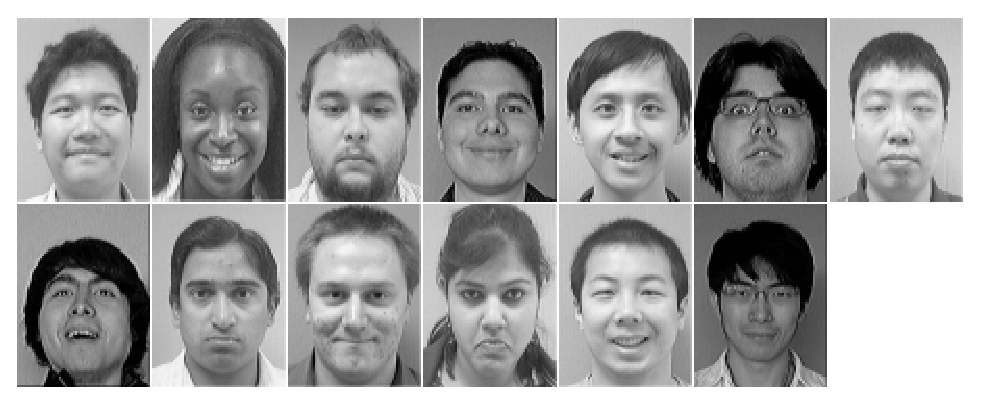
\includegraphics[width=3in]{figs/training_faces}
\begin{tabular}{c} \\[3ex] \end{tabular}
\begin{tabular}{|c|c|}
  \hline
  Person & Number of views\\
  \hline
  1 & 6\\
  2 & 7\\
  3 & 6\\
  4 & 22\\
  5 & 9\\
  6 & 16\\
  7 & 7\\
  8 & 22\\
  9 & 7\\
  10 & 7\\
  11 & 8\\
  12 & 7\\
  13 & 10\\
  14 & 53\\
  \hline
\end{tabular}
\caption{First view of the 14 people in the admissible set and the number of views for each person.  Person one is in the top left corner through person 14 in the lower right.}
\label{fig:training}
\end{figure}

The development network was built using 25 neurons in the Y layer and trained over 50 epochs of the training images.  For each epoch the optimal value for $R$ and $\theta$ were searched for using the grid search technique.  The search was performed over a subset of the input parameter space $R=[0.05-0.90]$ and $\theta=[0.05-0.90]$.  The sensitivity and specificity for each pair of values $R$ and $\theta$ were computed and plotted in a Receiver Operating Characteristics Curve, five representative epochs of which can be seen in \ref{fig:roc}. The network rapidly stabilized and achieved the best accuracy, $95.8\%$ after the third training epoch.  After the sixth training epoch the network achieved it's maximum sensitivity and specificity of $96.6\%$ and $92.5\%$ respectively with $R=.4$ and $\theta=.35$ and had an accuracy of $91.9\%$.  Beyond this point the sensitivity and specificity drop as the network began to over fit the training data.  

\begin{figure}
\center
\fontsize{8}{12}\selectfont
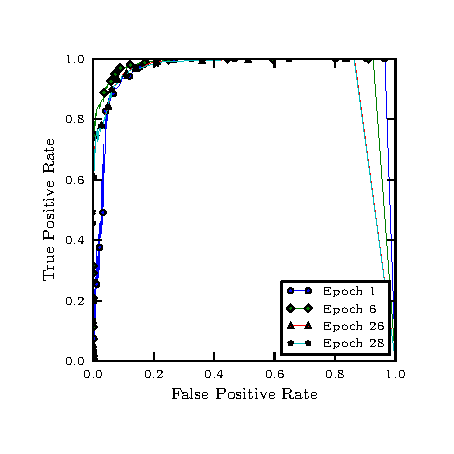
\includegraphics[width=2.75in]{figs/roc}
\caption{Receiver operating characteristic (ROC) curve for training epochs 1, 6, 9 and 26.  This figure shows how the sensitivity and specificity increase with the number of training epochs (curves shifting closer to the upper right hand corner) then fall off after the network begins over fitting.}
\label{fig:roc}
\end{figure}

The sixth training epoch, where the highest sensitivity and specificity were achieved, was analyzed further.  First the pre-synaptic weights for the $Y$ and $Z$ layer were visualized.  \ref{fig:y_weights} shows the pre-synaptic weights for the Y layer; these images are essentially averages of the input images that each neuron responds to.  Then the expected variation for each Y neuron, $\sigma$ was plotted in \ref{fig:y_sigmas}.  Each pixel represented the amount of variation the specific $Y$ neuron expects from the $X$ layer neuron.  Darker pixels represent lower expected variation while lighter pixels represent inputs with higher expected variation.  Of note is the first Y neuron, which is trained to respond to the background image that is presented before each classification task.  The image is a picture of the background each person had their picture taken against and the same image was presented each time which is why the expected variation is 0, an all black image.  For the Z layer the pre-synaptic weights for each of plotted in \ref{fig:z_weights} 5 per line. The lighter a square is the higher the weight for that Y neuron.  The firing ages for each of the Y and Z neurons were graphed in \${fig:ages} which showed that three neurons (neurons 2, 11, and 22) were under-utilized, responding to only a single view from the admissible set.  This is also shown in \ref{fig:y_sigmas} as the black squares, representing no expected variation in the input for those neurons.

\begin{figure}
\center
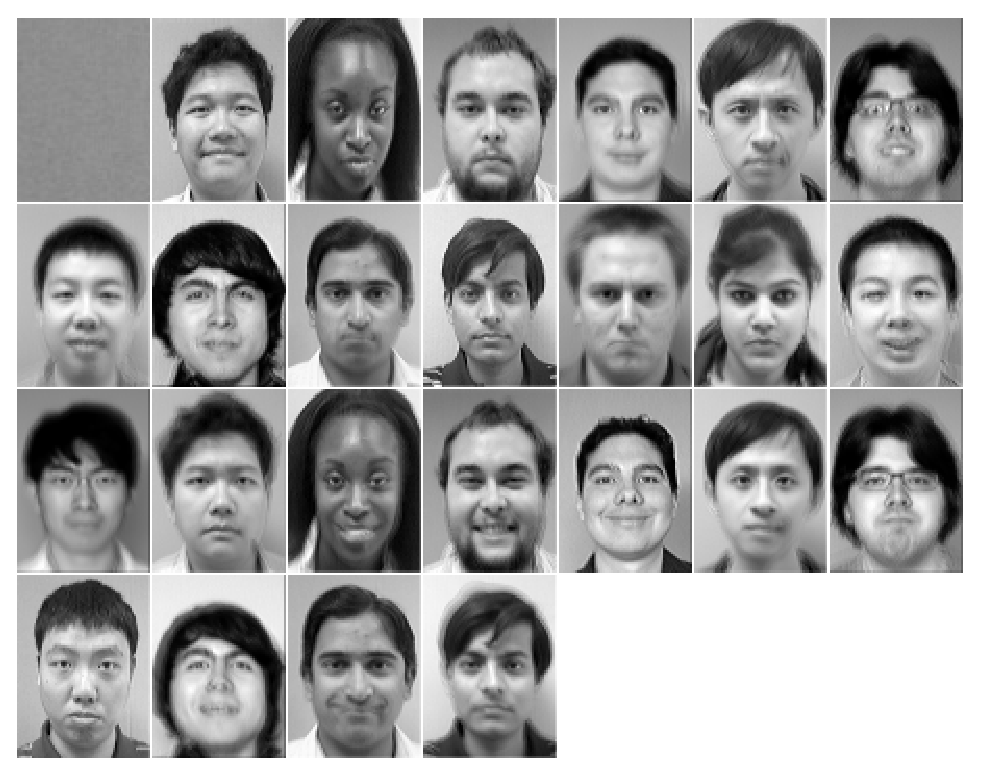
\includegraphics[width=3in]{figs/epoch_5_0_xy}
\caption{Visualization of pre-synaptic weights for the 25 Y layer neurons after the sixth training epoch, the first image corresponds to the Y neuron that responds to the background image presented to the network before every classification face.}
\label{fig:y_weights}
\end{figure}

\begin{figure}
\center
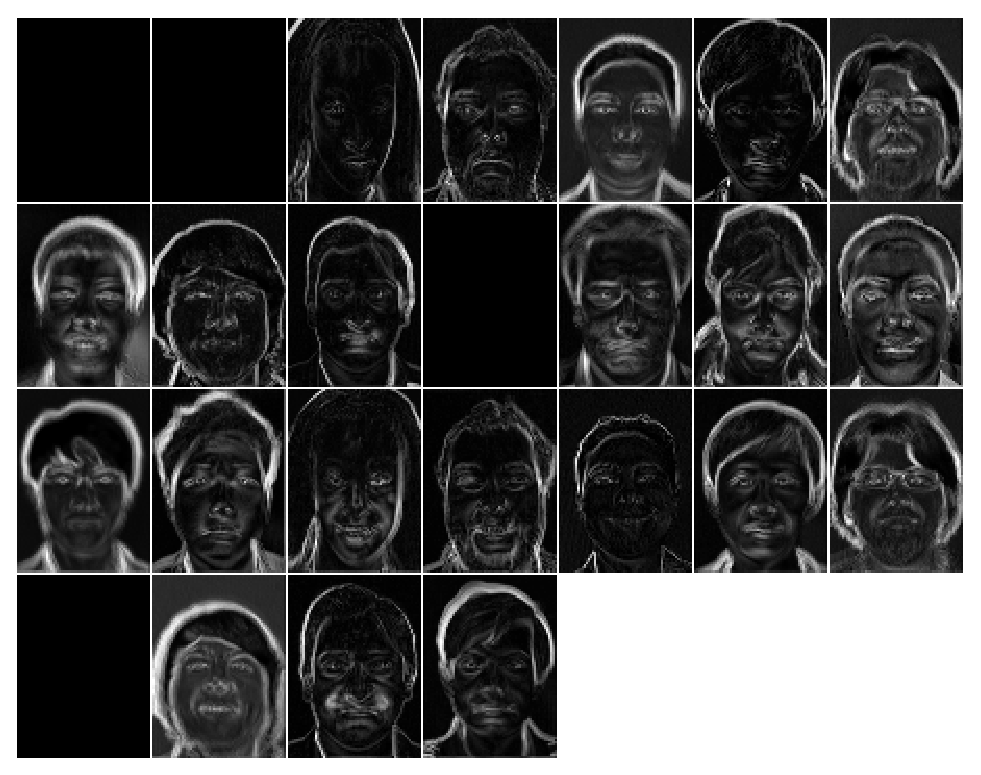
\includegraphics[width=3in]{figs/epoch_5_0_sigmas}
\caption{Visualization of the expected variance for each of the 25 neurons in the Y layer after the sixth training epoch.  The darker areas show inputs from the X layer where little variation is expected while the white areas show inputs that are expected to have larger variation.  Four neurons: 1, 2, 10, 22 (all black images) had no expected variation.}
\label{fig:y_sigmas}
\end{figure}

\begin{figure}
\center

\includegraphics[width=3in]{figs/epoch_5_0_yz}
\caption{Visualization of pre-synaptic weights for Z layer neurons after the sixth training epoch.  Each square represents a Z neuron.  The 25 pixels in each of the 25x25 squares represents the response weight for the corresponding Y neuron, the lighter the pixel the higher the weight.}
\label{fig:z_weights}
\end{figure}

\begin{figure}
\center
\fontsize{8}{12}\selectfont
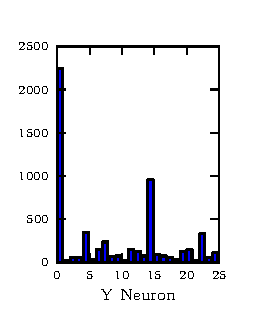
\includegraphics[width=1.5in]{figs/epoch_5_y_ages}
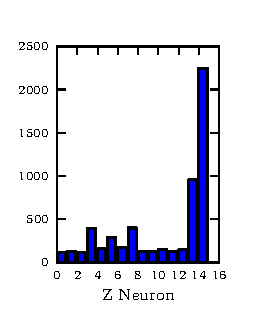
\includegraphics[width=1.5in]{figs/epoch_5_z_ages}
\caption{Plot of Y (left) and Z (right) neuron firing ages after the sixth training epoch.  The first (left most) Y neuron and last (right most) Z neuron are the neurons trained to respond to the background image that is presented before every image, which is why the firing rate for those neurons are higher than the rest.}
\label{fig:ages}
\end{figure}

Finally for the sixth epoch the 126 errors the network made when using the parameters $R=.4$ and $\theta=.35$ were broken down by error type: false acceptance, false rejection, and incorrect classification. Of the 126 errors a large number were duplicates of the same error, incorrectly classifying multiple views of the same person in to the same category.  Consolidating the errors down to one person input person-incorrect classification pair there were 3 false acceptances, 7 false rejections, and 2 incorrect classifications as seen in \ref{fig:6_epoch_errors}.  The falsely accepted faces on visual inspect appear very similar to people in the training set.  The false rejections appear to be a combination of mismatched white-balancing and errors made due to different facial expressions.  The mistakes appear to be due to facial expressions and orientations different from the learned faces.  The incorrect classifications and false rejections due to facial expressions can be improved by increasing the number of neurons in the Y layer.

\begin{figure}
\center
\begin{tabular}{cc}
\fontsize{8}{12}\selectfont
a \imagetop{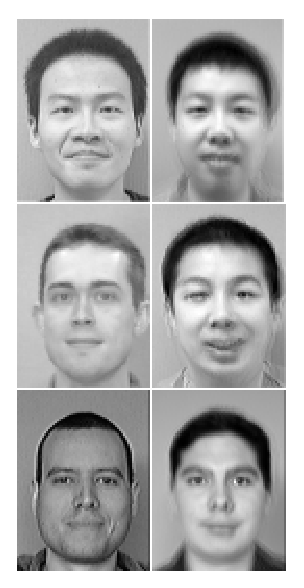
\includegraphics[width=1.4in]{figs/false_accept_combined}} &
\multirow{2}{*}{b \imagetop{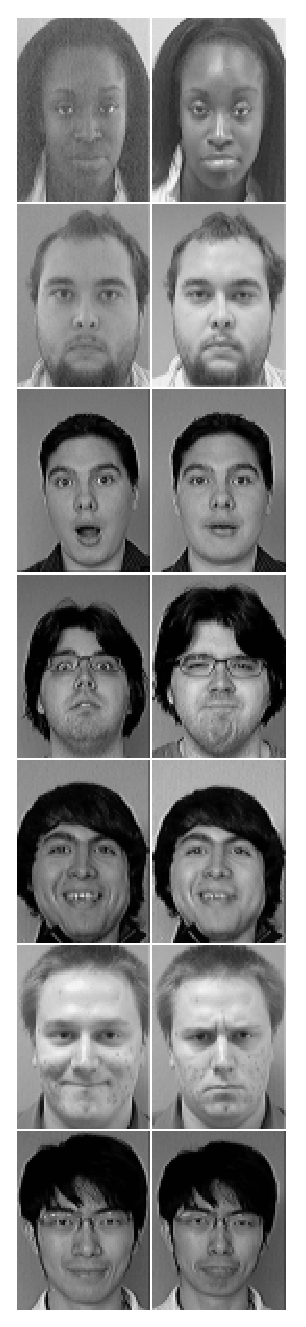
\includegraphics[width=1.4in]{figs/false_reject_combined}}} \\
c \imagetop{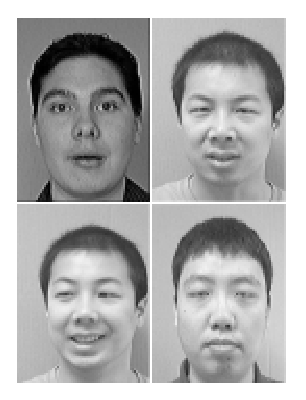
\includegraphics[width=1.4in]{figs/mistakes_combined}} & \\[60ex]
\end{tabular}
\caption{a. The incorrectly accepted image (on the left) compared to the y neuron pre-synaptic weights for the Y neuron with the highest response to the input image. b. Input image (left) compared to the first input face for the falsely rejected images. c. The input image (left) and view of the person (right) the network labeled the two misclassified people as.}
\label{fig:6_epoch_errors}
\end{figure}

\section{Conclusion}
The DN has been extended to include the Acetylcholine system and the Norepinenephrine system. 
By learning not only the patterns that come from each class but the expected distribution of the patterns this neural network is able to detect novel input patterns. The experiments here used images that are properly scaled and centered.   The future work is to apply the Ach and NE systems to the more general setting where
objects can appear at any location in a clutter background, as the Where-What Network \cite{WengNAI12}, an embodiment 
of DN, has been tested with but without the novelty detection mechanisms reported here. 


\label{SE:bib}
\bibliographystyle{plain}
%\bibliographystyle{Science}
\bibliography{shoslifref}

\end{document}  
